% \Stripe{offset}{color} long stripe
\newcommand\Stripe[2]{\draw[fill=#2,#2] ++(#1,0) +(-0.15,-0.71) rectangle +(0.15,0.71);}
% \stripe{offset}{color} short stripe
\newcommand\stripe[2]{\draw[fill=#2,#2] ++(#1,0) +(-0.15,-0.51) rectangle +(0.15,0.51);}

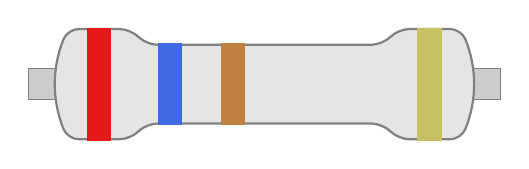
\begin{tikzpicture}
    % wire
    \draw[gray,fill=gray!40] (-3,-0.2) rectangle (3,0.2);
    % resistor
    \draw[rounded corners,thick,gray,fill=gray!20]
    ++(0,0.5) -- ++(1.5,0) -- ++(0.2,0.2) -- ++(0.8,0)
    .. controls +(0.2,-0.5) and +(0.2,0.5) .. ++(0,-1.4) -- ++(-0.8,0)
    -- ++(-0.2,0.2) -- ++(-3,0) -- ++(-0.2,-0.2) -- ++(-0.8,0)
    .. controls +(-0.2,0.5) and +(-0.2,-0.5) .. ++(0,1.4) -- ++(0.8,0)
    -- ++(0.2,-0.2) -- cycle;
    \Stripe{-2.1}{red!80!gray}
    \Stripe{2.1}{yellow!50!gray}
    \stripe{-1.2}{RoyalBlue}
    \stripe{-0.4}{brown}
\end{tikzpicture}